\section{The temperature for every day of the year}

%Part 3.2

To see the average trend of temperature throughout the year, we can average out the temperature for each date and add it to a histogram. The way this is implemented is by using a while loop that goes line by line of cleaned up .csv file. Within the while loop we check whether the current line has the same date as the previous, and if so we add the temperature to the running total, if not we find the mean of the previous running total and add it to the correct bin of the histogram. Due to this implementation, the last group of entries will not be added to the histogram, as the while loop would have to run again, but this is easy to fix because the necessary information is still stored in the variables. We address this by adding the last group of entries to the histogram outside the loop. Since all the mean temperatures are added to the bins, we need to then normalize the bin values by the number of weighted entries. We create a normalization array and in it count how many times a day was added to the histogram. See the plots in the Figures section. One can see that the climate is milder in cities that are not on or close to the coast. For example, it might be that Kiruna has the biggest spread of temperatures because the presence of mountains generally makes the weather harsher. 

\begin{table}[h]
    \centering
    \begin{tabular}{|c|c|c|} \hline
        City  & Max & Min \\ \hline
        Lund & 14.3896 & 1.35988 \\
        Falsterbo & 15.2263 & 1.98313 \\
        Kiruna & 13.4096 & -14.0109 \\
        Göteborg & 14.6356 & 1.43963 \\
        Gävle & 13.8721 & -2.83569 \\
        Jönköping & 12.6589 & -0.163235 \\
        \hline
        
    \end{tabular}
    \caption{Maximum and minimum mean temperatures in different cities}
    \label{tab:my_label}
\end{table}

\begin{figure}
    \centering
    \begin{subfigure}[b]{0.49\textwidth}
    \centering
    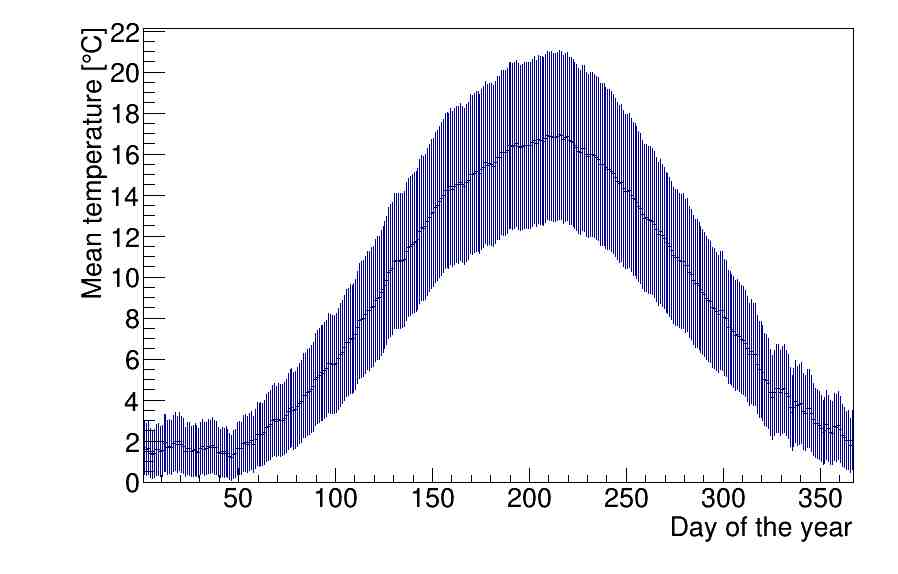
\includegraphics[width=\textwidth]{FAL_A.jpg}
        \caption{Falsterbo}
    \end{subfigure}
    \hfill
    \begin{subfigure}[b]{0.49\textwidth}
    \centering
    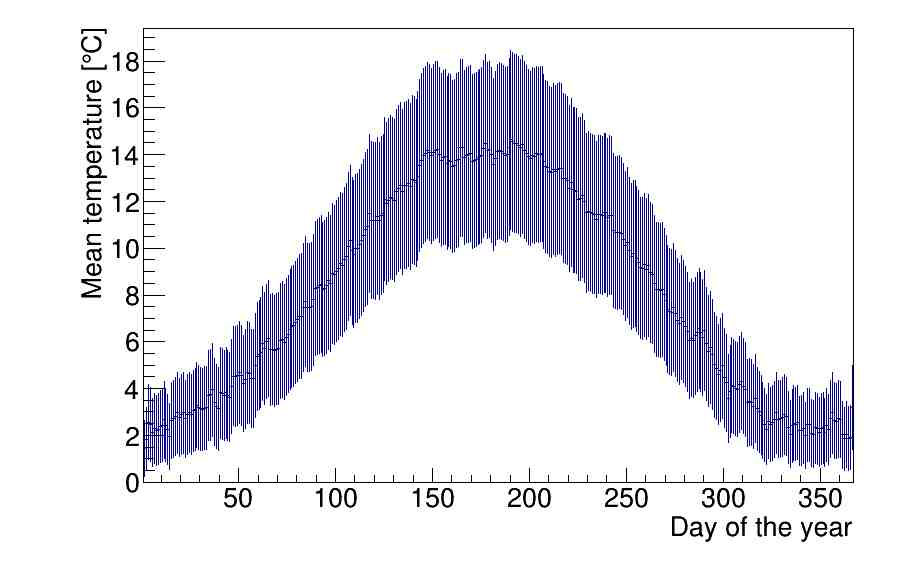
\includegraphics[width=\textwidth]{GBG_A.jpg}
        \caption{Göteborg}
    \end{subfigure}
    
    \begin{subfigure}[b]{0.49\textwidth}
    \centering
    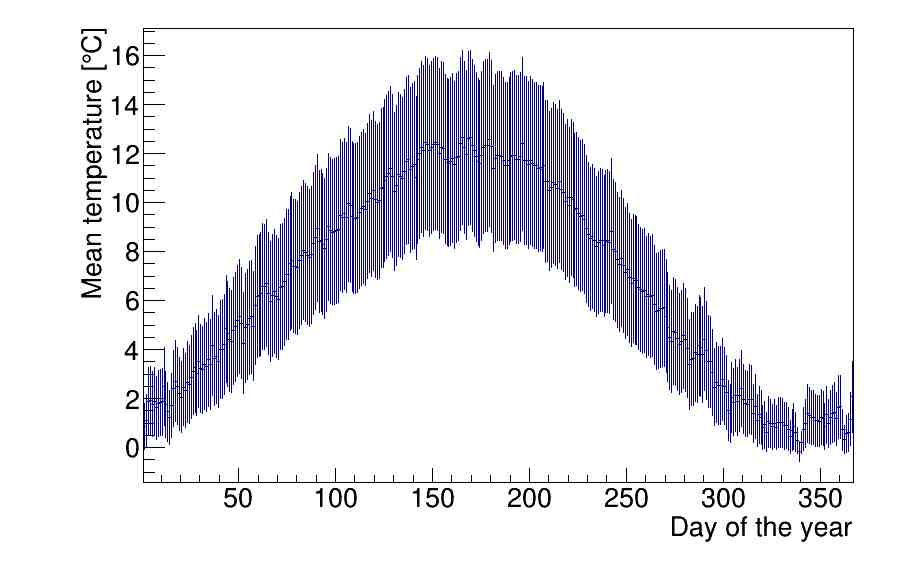
\includegraphics[width=\textwidth]{JKP_A.jpg}
        \caption{Jönköping}
    \end{subfigure}
    \hfill
    \begin{subfigure}[b]{0.49\textwidth}
    \centering
    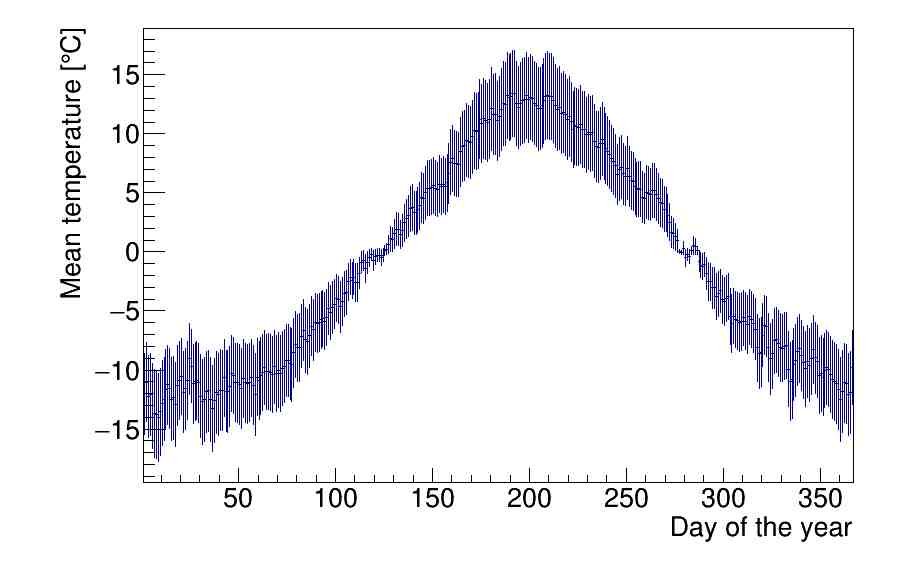
\includegraphics[width=\textwidth]{KIR_A.jpg}
        \caption{Kiruna}
    \end{subfigure}
    \begin{subfigure}[b]{0.49\textwidth}
    \centering
    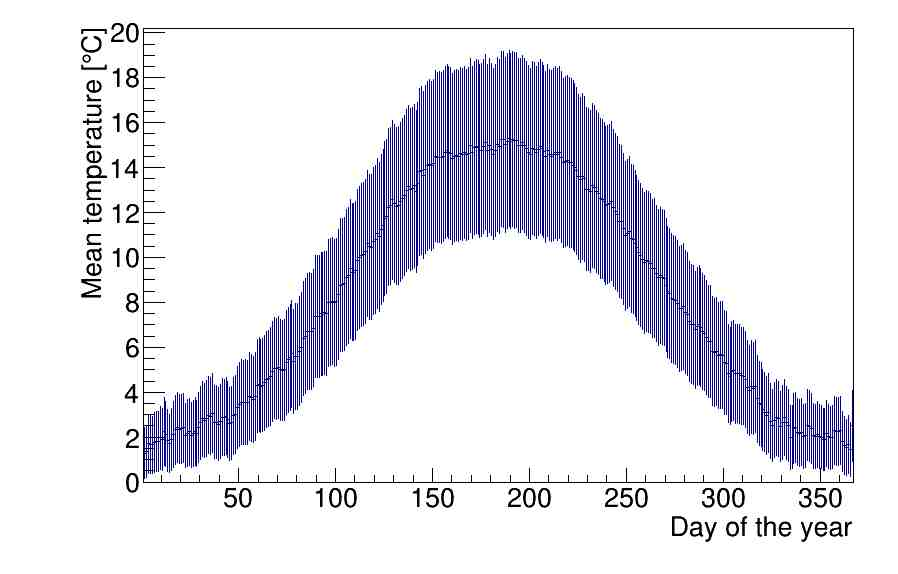
\includegraphics[width=\textwidth]{LU_A.jpg}
        \caption{Lund}    
    \end{subfigure}
    \hfill
    \begin{subfigure}[b]{0.49\textwidth}
    \centering
    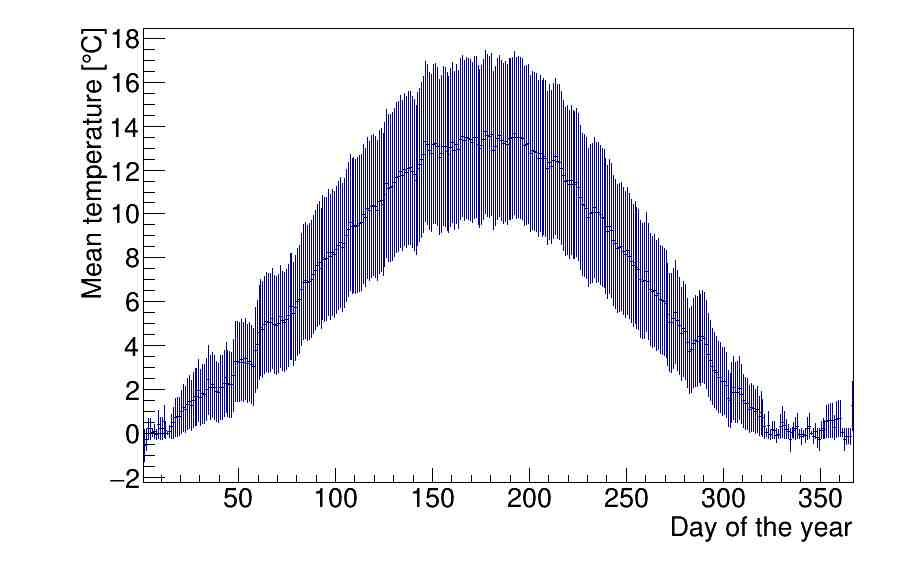
\includegraphics[width=\textwidth]{STH_A.jpg}
        \caption{Stockholm}    
    \end{subfigure}
\end{figure}




%Lund: Max: 14.3896, Min: 1.35988 
%Falsterbo: Max: 15.2263, Min: 1.98313
%Kiruna : Max: 13.4096, Min: -14.0109
%Göteborg: Max: 14.6356, Min: 1.43963
%Gävle: Max: 13.8721, Min: -2.83569
%Jönköping: Max: 12.6589, Min: -0.163235

